\documentclass[a4paper,11pt]{article}
\pagestyle{headings}

\usepackage[utf8]{inputenc}
\usepackage{diagbox}
\usepackage[french]{babel}
\usepackage{graphicx}
\usepackage{float}
\usepackage{fullpage}
\usepackage{hyperref}
\usepackage{diagbox}
\usepackage{enumitem}
\usepackage[T1]{fontenc}
\usepackage[]{algorithm2e}
\usepackage{url}
\usepackage{array}
\usepackage{amsmath}
\graphicspath{{images/}}

\title{Reconnaissance de formes et apprentissage automatique Projet 3}
\author{Auriane Reverdell, Felix Hähnlein, Nicolas Violette, Romain Duléry}
\date{\today}

\setlength{\oddsidemargin}{0.2cm}
\setlength{\evensidemargin}{-0.7cm}
\setlength{\parindent}{30pt}
\setlength{\textwidth}{15cm}
\setlength{\textheight}{24cm}
\setlength{\topmargin}{-.3in}
\setlength{\parskip}{1ex}


\begin{document}

\maketitle
\vspace{1cm}

\section{Problématique}
    
    La problématique de ce projet est d'évaluer la performance d'un réseau de neurones profond. Dans
    notre cas, nous avons cherché à comparer deux méthodes : entraîner le réseau sur notre propre
    jeu de données ou encore faire du transfer-learning (i.e. prendre un réseau pré-entraîner et
    faire l'entraînement des dernières couches. Nous avons aussi expérimenté l'augmentation de données
    car la performance de l'algorithme est grandement dépendante du jeu de données d'entraînement.

\section{Utilisation de notre propre réseau de neurones}

    Pour se rendre compte de l'éventail des difficultés liées au Deep Learning et afin de mieux comprendre son fonctionnement, il est important d'implémenter et d'entraîner son propre réseau de neurones.
    En effet, nous pouvons distinguer deux étapes bien différentes, la construction du réseau de neurones et son entraînement.

\subsection{Construction du réseau de neurones}
    
    Le choix du design d'un réseau de neurones est loin d'être une tâche triviale.
    Selon la problématique, la taille des données d'entrée et le temps que nous avons à notre disposition, l'architecture appropriée peut largement varier.
    Même pour un problème donné, les architectures ont beaucoup varié pendant les dernières décennies, grâce à l'amélioration du matérial utilisé et la programmabilité croissante du GPU.
    Effectivement, la complexité d'un réseau de neurones est directement liée au temps d'entraînement ce qui nous conduit à opter pour des réseaus plus profonds et des couches plus larges pendant ces dernières années.
    \\
    Alors qu'il est difficile de théoriser l'architecture à choisir, nous pouvons quand même faire quelques remarques par rapport à notre problème:
    \begin{itemize}
        \item
            Nous avons au moins besoin de 3 couches convolutionnelles si nous voulons détecter des feautures de bas niveau, moyen niveau et haut niveau.
            Ce comportement a été montré dans les travaux de Zeiler et al. \cite{zeiler2014visualizing}.
            Chacune de ces couches se construit par aggrégation de parties de la couche précédente.
        \item
            Après les couches convolutionnelles, nous retrouvons souvent au moins une couche complètement connectée avec un nombre de neurones important.
            Cette couche sert à mettre en relation les features de haut niveau. 
            Par exemple, un visage dispose de 2 yeux alignées.
            Tandis que la couche convolutionnelle de haut niveau va détecter la présence d'un oeil, la couche complètement connectée va pouvoir nous dire si nous en avons deux juste au-dessus du nez.
        \item
            En sortie de la toute dernière couche, nous retrouvons autant de neurones que de classes à distinguer.
            Ici, il est important à noter que le problème de détection peut être considéré comme un problème de détection appliqué à des sous-images.
            Par rapport à notre problème, cela veut dire que nous avons deux neurones de sortie, donnant la probabilité que l'imagette appartient à un visage ou pas.
    \end{itemize}

    Étant donné qu'il s'agit de notre première expérience construction de réseaux de neurones, nous nous sommes fortement inspirés d'un réseau d'un projet \textit{GitHub} \cite{face_detect} existant, accomplissant la même tâche avec approximativement la même taille de données d'entrée.
    \\
    L'architecture utilisée est resumée dans la table \ref{tab:network_architecture}. Le réseau prend en entrée des imagettes de taille $32\times32$.
    \\
    En plus des considérations précédentes, nous pouvons remarquer que chaque couche convolutionnelle est suivie d'une couche de sous-échantillonnage qui sert à réduire le nombre de paramètres filtrant les plus importants.
    \begin{table}
        \begin{tabular}{|l|c|c|c|c|c|c|c|r|}
            
            \hline
            \textbf{Layer} & Conv1 & MaxPool & Conv2 & MaxPool & Conv3 & MaxPool & Fc1 & Fc2 \\
            %colonne 1 & colonne 2 & colonne 3 & colonne 4 \\
            \hline
            \textbf{Kernel Size} & 5x5 & 2x2 & 3x3 & 2x2 & 3x3 & 2x2 & -  & - \\
            \textbf{Features} & 4 & - & 16 & - & 32 & - & 600  & 2 \\
            \hline
        \end{tabular}
        \caption{Architecture du réseau de neurones}
        \label{tab:network_architecture}
    \end{table}

\subsection{Paramètres d'entraînement}

    Pour nos premières expériences d'entraînement, nous avons utilisé des paramètres d'entraînement communément utilisé dans le cadre du framework \textit{Tensorflow}.
    \begin{itemize}
        \item{\textit{Fonction d'activation}} Softmax
        \item{\textit{Fonction de coût}} Entropie croisée
        \item{\textit{Taux d'apprentissage}} \verb$1e-4$
        \item{\textit{Taille des batchs}} $100$
    \end{itemize}

\subsection{Entraînement du réseau de neurones}
    
    Pendant l'entraînement du réseau, il est important de pouvoir le diagnostiquer.
    Pour cela, il est utile d'afficher la précision d'entraînement et la précision de test.
    Ce que nous entendons ici par précision, c'est en fait l'\textit{accuracy} qui est donnée par $\frac{TP+TN}{TP+FP+TN+FN}$.
    Il s'agit du ratio de bonnes classifications.
    %Alors que cette métrique n'est peut-être pas la métrique la plus représentative 
    Cette métrique a deux avantages. 
    Premièrement, elle tient compte du problème de classification que nous voulons résoudre.
    Deuxièmement, elle est facile à obtenir, car elle est calculée directement à la sortie du réseau de neurones pour le calcul de la fonction de coût.
    \\

    Quand nous proposons un modèle, nous sommes toujours confronté à la question de savoir s'il comporte trop de paramètres ou s'il n'y en a pas assez, compte-tenu de la complexité du problème.
    On dit qu'on est confronté à un problème de \textit{sur-ajustement} ou de
    \textit{sous-ajustement} (\textit{overfitting} ou \textit{underfitting}).
    L'affichage des deux précisions nous permet de savoir dans lequel des deux cas on se trouve.
    Sur la figure \ref{fig:overfitting_1}, nous constatons que la précision de test diminue, alors que celle d'entraînement ne cesse d'augmenter.
    En plus, les oscillations de la courbe de précision de test indiquent que le modèle utilisé n'arrive pas à généraliser les informations d'entrée de manière fiable.
    Nous sommes alors confrontés à un problème de sur-ajustement.
    Pour résoudre ces problèmes, nous avons appliqué des méthodes de régularisation (voir la section
    \ref{sec:regularization}).

	\begin{figure}[H]
	    \centering
	    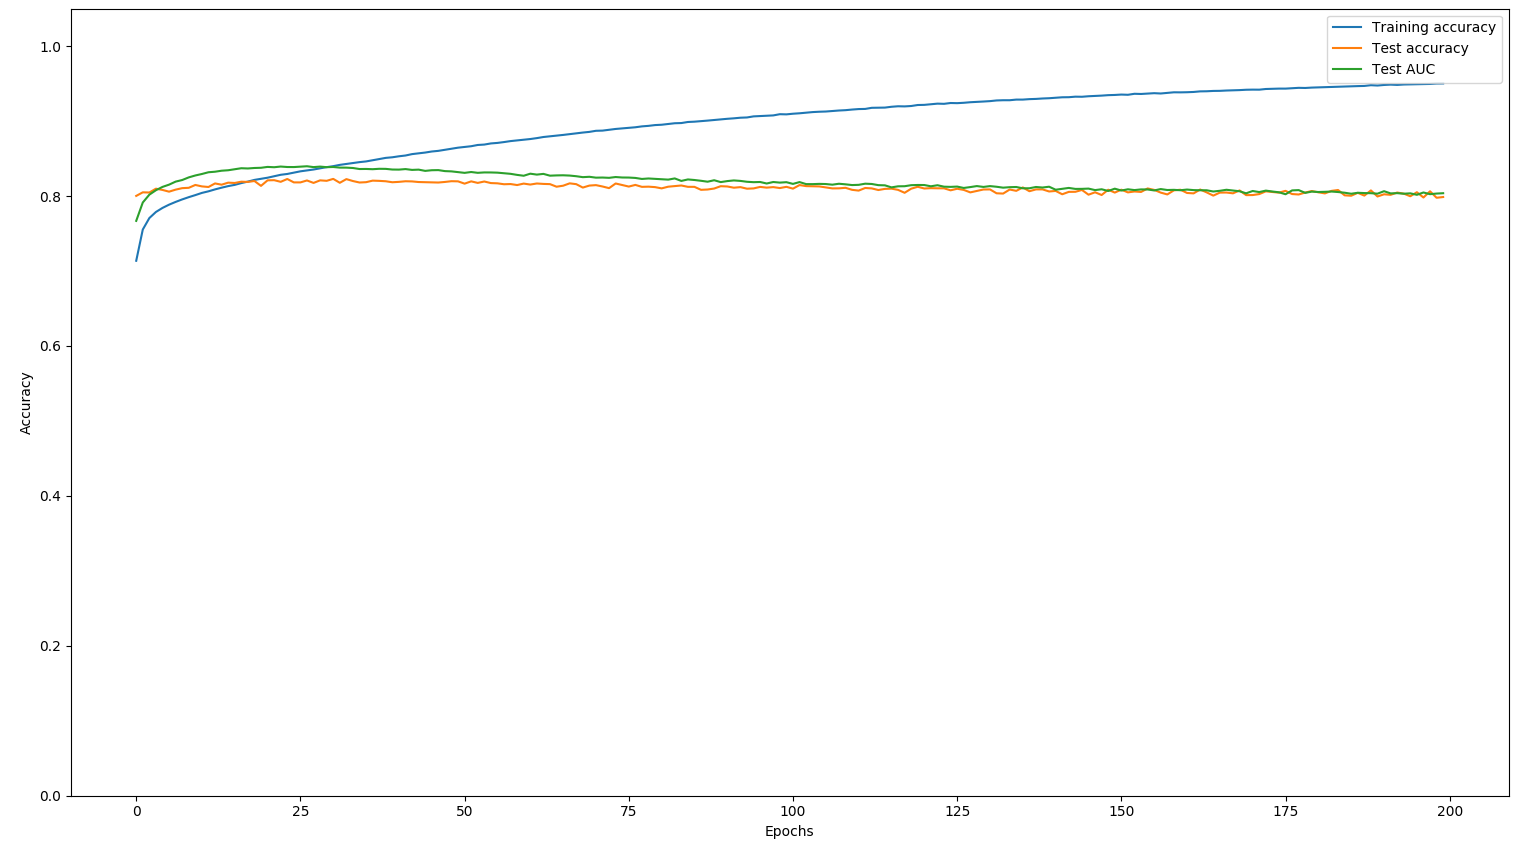
\includegraphics[scale=0.3]{overfitting_1.png}
	    \caption{Graphe des deux précisions. Nous sommes confrontés à un sur-ajustement du modèle.}
	    \label{fig:overfitting_1}
	\end{figure}

\subsection{Méthodes de régularisation}
\label{sec:regularization}
    
    Pendant la phase d'entraînement, nous avons besoin de pouvoir diagnostiquer le comportement du réseau.
    Pour mieux comprendre la régularisation d'un réseau de neurones, il est utile de se rappeler son fonctionnement.
    Un réseau de neurones est une méthode d'optimisation.
    Grâce à l'algorithme de \textit{rétropropagation du gradient}, il arrive à minimiser la fonction
    du coût en modifiant les poids et les biais.
    Autrement dit, l'algorithme cherche la meilleure solution dans l'espace des vecteurs de poids pour une fonction de coût donnée.
    Lors du sur-ajustement, quelques éléments de ce vecteur peuvent être disproportionnés par
    rapport au reste, il est alors biaisé dans une certaine direction.
    L'algorithme d'optimisation va alors plus difficilement pouvoir explorer d'autres directions de l'espace de solutions.
    \\
    Les méthodes de régularisation visent à limiter la présence de ces poids abbérants.
    Nous avons testé les deux méthodes suivantes. 
    \begin{itemize}
        \item{\textit{Dropout}}

            La technique de dropout simule le disfonctionnement naturel temporaire de nos neurones.
            Elle s'applique à une ou plusieurs couches du réseau où elle enlève aléatoirement un certain nombre des neurones.
            Cela favorise la participation égale de toutes les neurones de la couche.
            Une illustration de cette méthode se trouve sur la figure \ref{fig:dropout_illustration}. 

        \item{\textit{La pénalisation des poids}}
            La méthode de pénalisation des poids consiste à rajouter un terme auxiliaire à la fonction de coût qui dépend de manière directe de la norme des poids du réseau.
            Voici un exemple de pénalisation de poids pour la norme $\mathcal{L}^2$.
            \begin{equation*}
                c = c_0 + \frac{\lambda}{n}\sum_{i=1}^n w_i^2
            \end{equation*}
        Remarquons que cette méthode va uniquement régulariser le réseau au sens de la norme utilisée.
    \end{itemize}

    Nous avons implémenté ces deux méthodes.
    Les résultats de la méthode de dropout se trouvent sur les figures \ref{fig:overfitting_with_dropout} et \ref{fig:overfitting_without_dropout}.
    Nous constatons que le sur-ajustement commence plus tard, environ à partir de l'époque 15 au
    lieu de l'époque 5 (sans dropout), que le même taux de précision est atteint plus rapidement
    avec dropout et que la précision de test a globalement augmenté.
    \\
    Sur la figure \ref{fig:l2_regularization}, nous avons visualisé les résultats de l'entraînement en utilisant la deuxième méthode.
    Nous n'obtenons plus de sur-ajustement et la valeur des AUC (\textit{area under the curve})
    augmente jusqu'à $0.891$ pour notre ensemble de test.
    À partir de l'époque 100, nous remarquons que les deux courbes sont plafonnées, alors qu'on obtient des performances comparables au premier projet qui utilisait des histogrammes RGB.
    Ce phénomène de saturation nous indique qu'on est maintenant confronté à un problème de sous-ajustement qui va être décrit dans la section \ref{sec:sous-ajustement}.

	\begin{figure}[H]
	    \centering
	    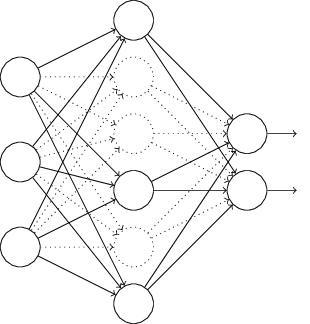
\includegraphics[scale=0.5]{dropout_illustration.png}
	    \caption{Illustration de la méthode de dropout. Les neurones en pointillés ne vont pas être "oubliés".}
	    \label{fig:dropout_illustration}
	\end{figure}

	\begin{figure}[H]
	    \centering
	    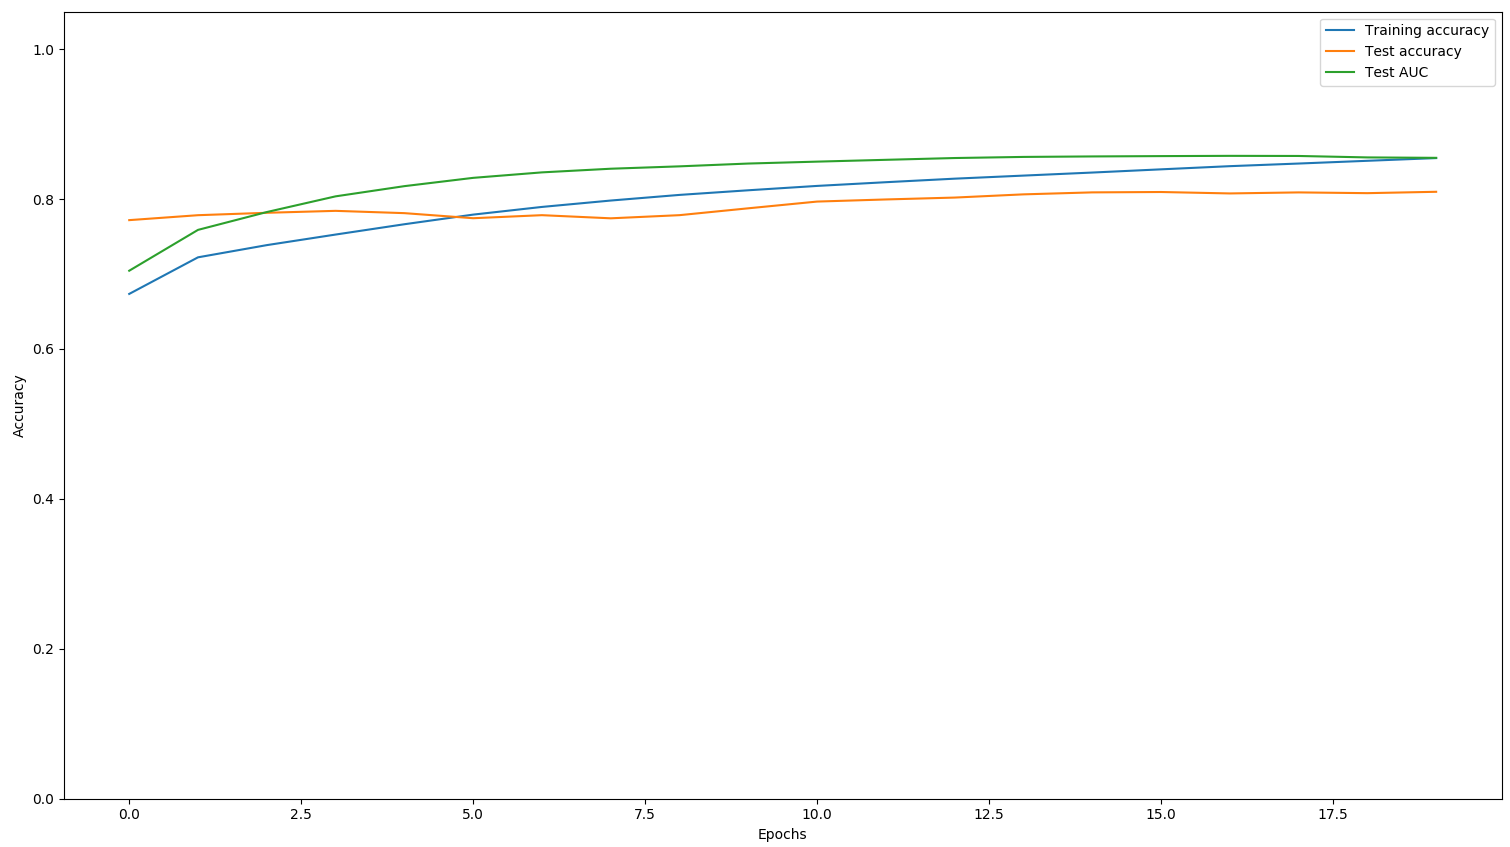
\includegraphics[scale=0.3]{overfitting_without_dropout.png}
	    \caption{Entraînement sans dropout}
	    \label{fig:overfitting_without_dropout}
	\end{figure}

	\begin{figure}[H]
	    \centering
	    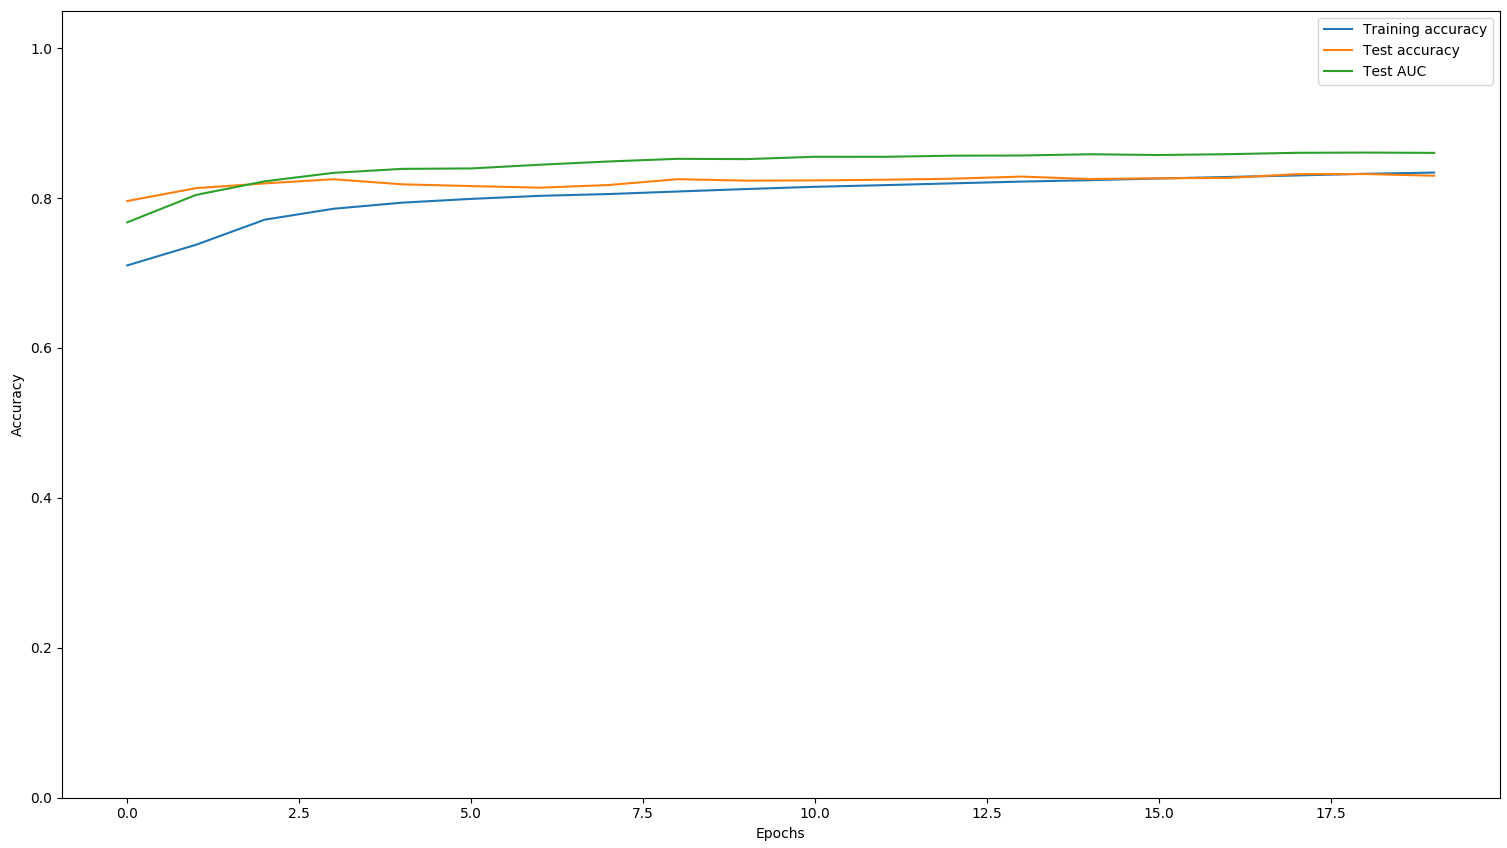
\includegraphics[scale=0.3]{overfitting_with_dropout.png}
	    \caption{Entraînement avec dropout}
	    \label{fig:overfitting_with_dropout}
	\end{figure}

	\begin{figure}[H]
	    \centering
	    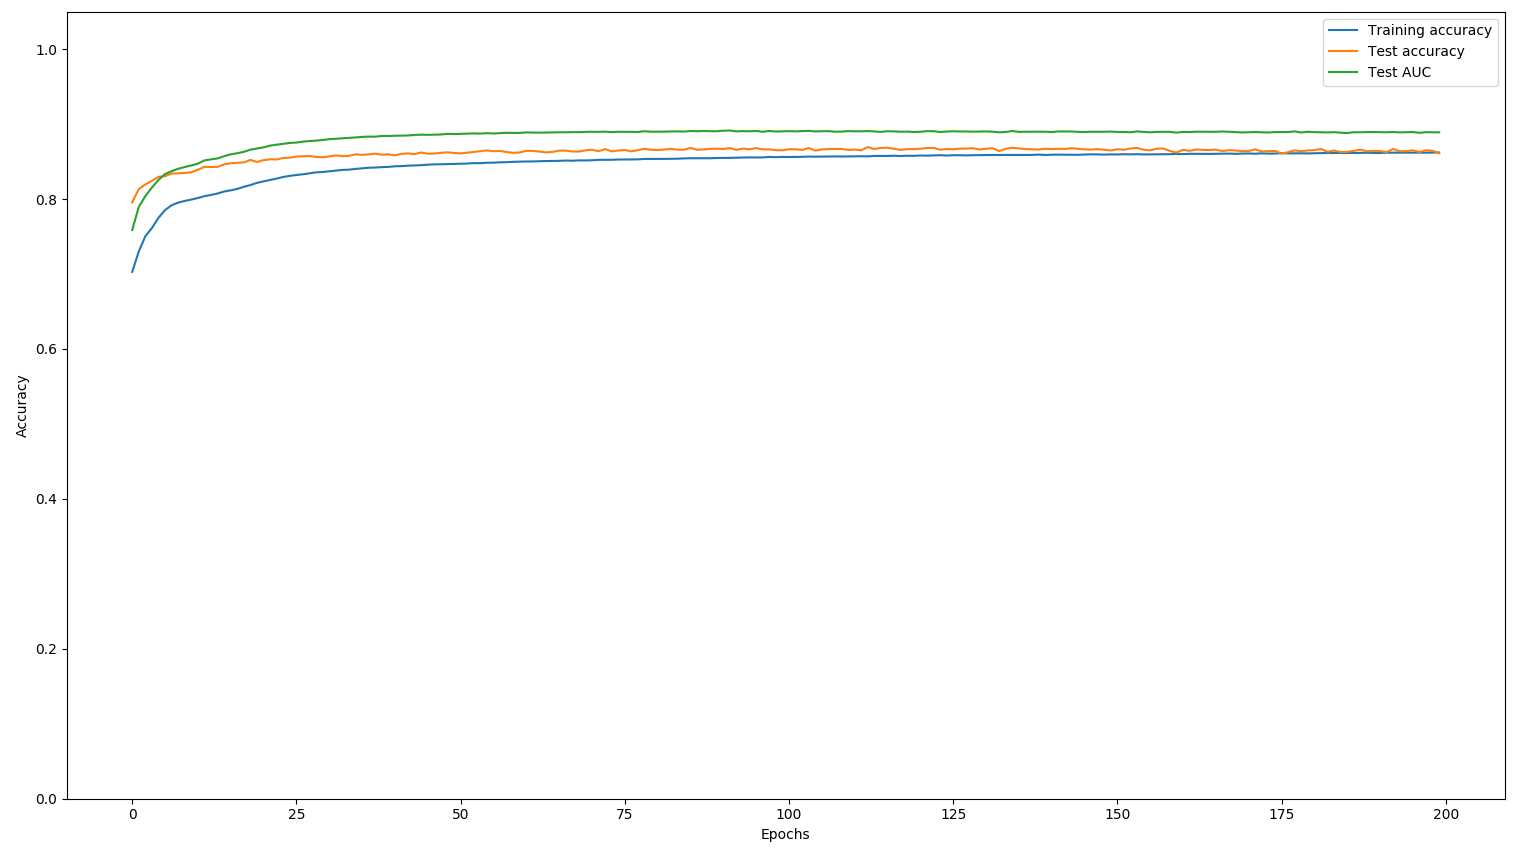
\includegraphics[scale=0.3]{l2_regularization_200.png}
	    \caption{Entraînement avec pénalisation de poids $\mathcal{L}^2$}
	    \label{fig:l2_regularization}
	\end{figure}

\subsection{Sous-ajustement}
\label{sec:sous-ajustement}

    Nous sommes face à un problème de sous-ajustement dans un des deux cas suivants :
    \begin{itemize}
        \item 
            Notre modèle n'est pas assez complexe, i.e. ne comporte pas assez de paramètres, pour modéliser les données.
            Dans ce cas, il suffit d'augmenter la complexité du réseau de neurones, c'est-à-dire d'ajouter des couches ou d'augmenter le nombre de features par couche.
            Nous avons complexifié l'architecture de notre réseau, mais cela n'a pas augmenté sa performance.

        \item
            Les données utilisées pour l'entraînement ne sont pas assez représentatives pour modéliser le problème.
            Cela signifie dans notre cas, que des simples imagettes de taille $32\times32$ ne contiennent pas assez d'informations pour mener notre algorithme à la bonne décision.
            Nous avons pu vérifier cette hypothèse avec la méthode de \textit{transert learning} décrite dans la section \ref{sec:transfert_learning}.
            Nous avons entraîné un réseau avec deux tailles d'imagettes différentes.
            La précision finale est nettement meilleure avec des imagettes plus grandes en entrée. 
    \end{itemize}

    Nous nous sommes rendus compte que la détection basée sur des parties trop petites du visage pose des problèmes.
    Pour pallier le problème d'ajustement de la taille des imagettes, nous avons implémenté une
    pyramide d'images, comme suggéré par un groupe lors des présentations.

\subsection{Pyramide d'images}

    L'idée de la pyramide d'images est de ne plus traiter l'image qu'à l'échelle originale, mais de traiter un ensemble d'images composé de l'image d'entrée à plusieurs échelles.
    L'avantage de cette structure par rapport à notre problème est que nous pouvons donner des visages entiers à notre réseau de neurones.
    Étant donné que l'imagette contient tout le visage, le réseau aura toutes les informations nécessaires pour prendre une décision.
    \\
    En pratique, nous extrayons tous les visages de la base de données \textit{WIDER} que nous redimensionnons.
    Ces images constituent notre ensemble d'images positives.
    Pour construire l'ensemble négatif, nous prenons un patch n'appartenant pas à une région de visage au hasard pour chaque visage extrait précédemment.
    À part des données d'entrées, nous n'avons rien changé par rapport à l'entraînement précédent.

\subsubsection{Détection de visages}
    
    Après avoir entrainé notre réseau, nous devons changer la manière que nous détectons des visages sur des nouvelles images.
    Pour cela, nous parcourons l'image à plusieurs échelles et nous redimensionnons les détections positives.
    Nous avons alors en sortie un ensemble de rectangles, que nous regroupons en utilisant la fonction \verb$groupRectangles$ de \textit{OpenCV}.

\subsubsection{Résultats}

    Nous avons entrainé le réseau sur 200 époques et nous l'avons appliqué à des images provenant de la base de données \textit{FDDB}.
    Des exemples testés se trouvent sur les figures \ref{fig:first_scale} à \ref{fig:last_scale}.

	\begin{figure}[H]
	    \centering
	    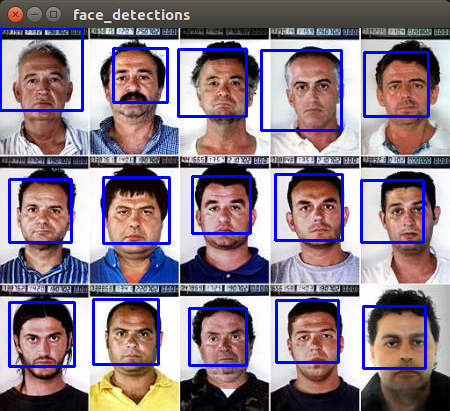
\includegraphics[scale=0.3]{first_scale.png}
	    \caption{Visages multiples évalués avec la pyramide d'images}
	    \label{fig:first_scale}
	\end{figure}
	\begin{figure}[H]
	    \centering
	    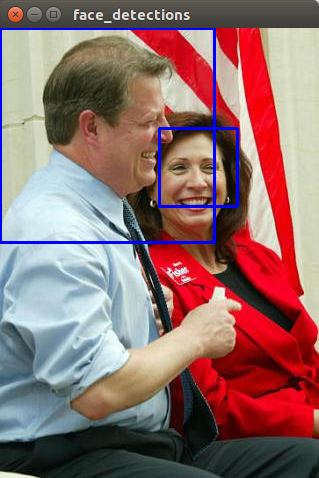
\includegraphics[scale=0.3]{scale_2.png}
	    \caption{Visages proches évalués avec la pyramide d'images}
	    \label{fig:scale_2}
	\end{figure}
	\begin{figure}[H]
	    \centering
	    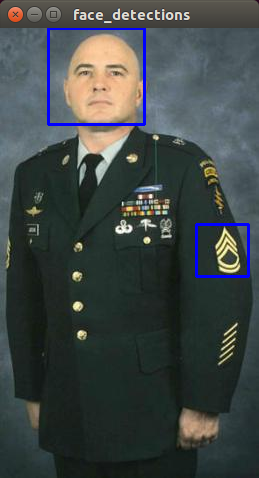
\includegraphics[scale=0.3]{scale_3.png}
	    \caption{Image évaluée avec la pyramide d'images}
	    \label{fig:scale_3}
	\end{figure}

    Nos tests nous montrent qu'on a obtenu une bonne amélioration grâce à l'utilisation de la pyramide d'images.
    En plus de cela, le regroupement des détections positives filtre davantage les faux positifs.
    Un exemple sans filtrage se trouve sur la figure \ref{fig:without_filter}.

	\begin{figure}[H]
	    \centering
	    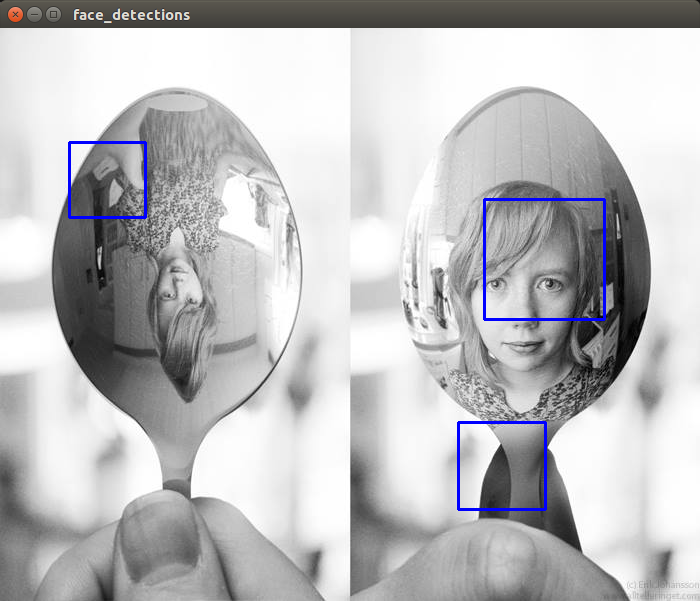
\includegraphics[scale=0.3]{last_scale.png}
	    \caption{Robustesse de l'algorithme sur une déformation}
	    \label{fig:last_scale}
	\end{figure}

	Nous pouvons voir ici que notre algorithme n'est pas robuste aux déformations, cela vient du
	fait que nous n'avons pas augmenté nos données d'entraînement sur les déformations.


	\begin{figure}[H]
	    \centering
	    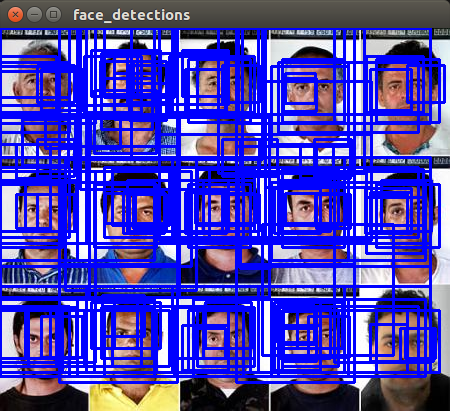
\includegraphics[scale=0.3]{without_filter.png}
	    \caption{Figure \ref{fig:first_scale} sans regroupement de rectangles}
	    \label{fig:without_filter}
	\end{figure}


\section{Visualisation du réseau de neurones}
\subsection{Principes et méthode}
A des fins d'évaluations du bon fonctionnement de notre réseau, nous nous sommes également
penché sur le papier de Matthew D. Zeiler et Rob Fergus (2013) qui traite de la visualisation d'un réseau de neurones.
Nous avons téléchargé et adapté à notre code source un dépôt github qui implémente une partie
de ce qui est traité dans ledit papier. Cette technique utilise une inversion du principe des
réseaux de neurones convolutionnels (les "deconvolutionnal networks") pour inverser la navigation entre les
couches et ainsi pouvoir générer une visualisation meme pour les niveaux éloignés qui ne sont pas facilement
reliable avec les pixels d'entrée. Cette technique n'est pas sans perte car la reconstruction tient seulement
compte des neurones particulièrement activés lors du passage d'une seule window dans le réseau.
Ceci est néanmoins suffisant pour avoir un rendu correct.

\subsection{Application}
Lors de l'application de ceci sur notre réseau, on obtient les images suivantes :

\begin{figure}[H]
    \centering
    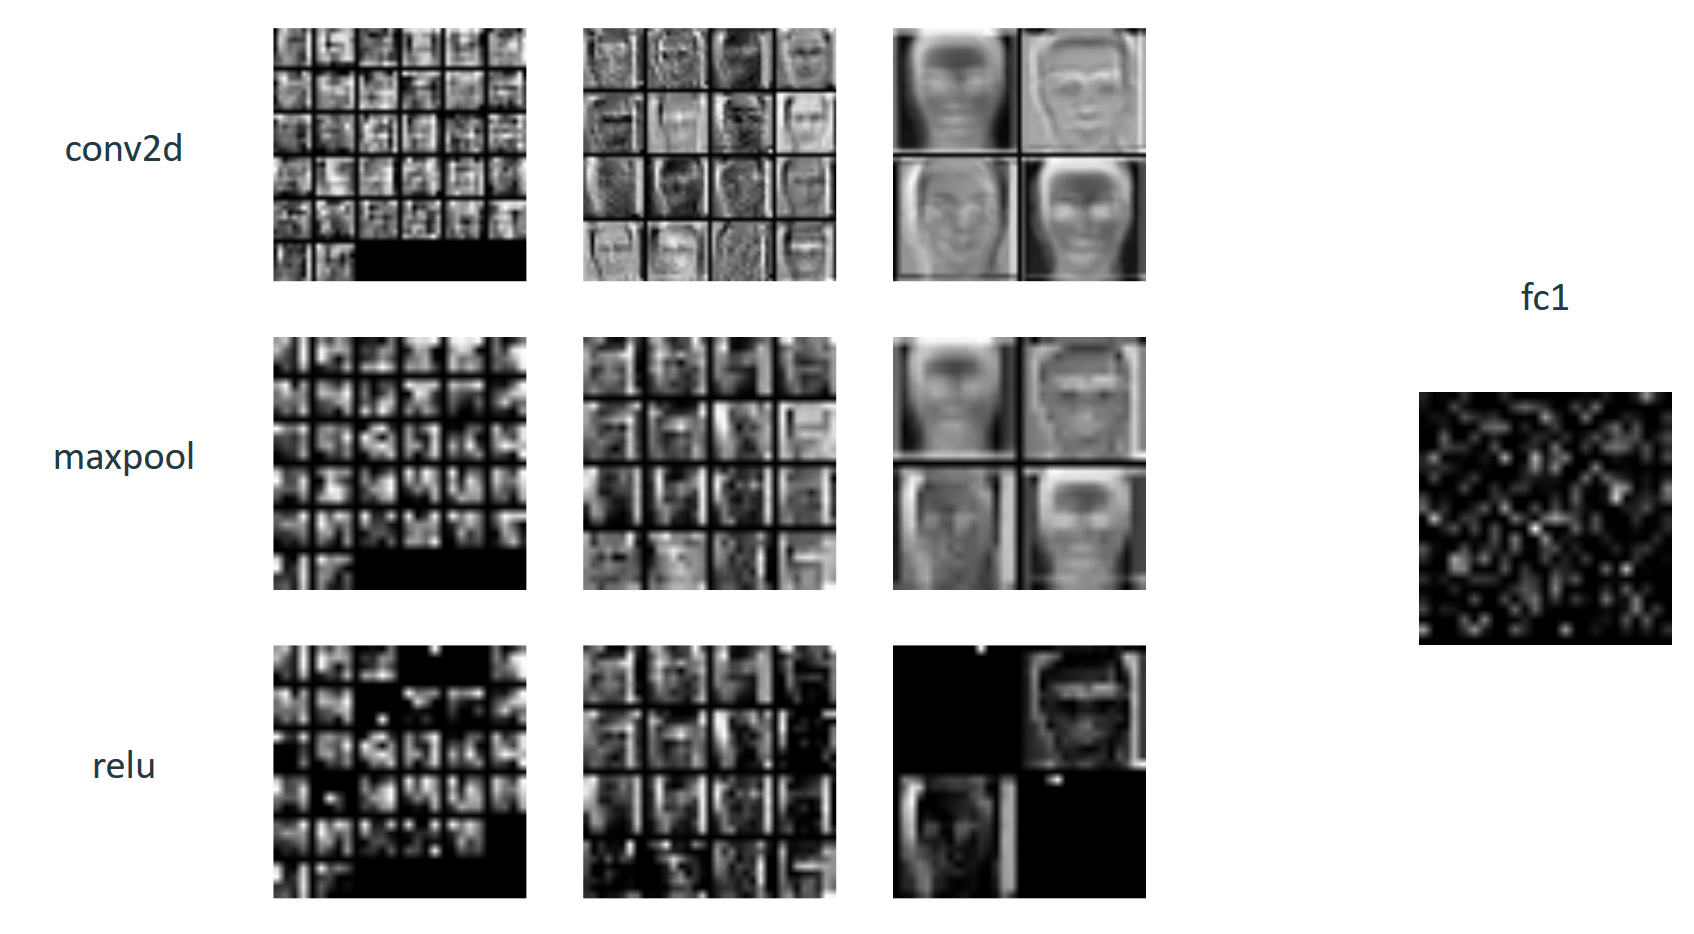
\includegraphics[scale=0.25]{visu.png}
    \caption{Visualisation des neurones activés pour chaque fonction de chaque couche}
    \label{fig:visu}
\end{figure}

On peut voir que la reconstruction d'une image aux différents niveaux du réseau se fait bien, malgré les difficultés
théoriques précédemment mentionnées. En revanche, là où l'on s'attendrait à voir en première couche des petites features
méconaissables (des traits, des arrêtes, des tâches, etc.), en deuxième couche une composition de ces features pour
réagir à des éléments plus important (yeux, nez, bouche, machoire, etc.), et en dernière couche des visages; on se
retrouve en fait avec un simple downscaling de la window à chaque couche.
On notera en revanche que les différentes opérations à chaque niveau s'effectuent correctement, et que le rendu est
cohérent à celui que l'on s'attendrait à obtenir en théorie (par exemple, le max pooling a bien un effet de
réduction d'échelle sur l'image résultante, qui apparaît donc "pixellisée").

Nous avons également essayé d'implémenter des fonctionnalités de "deepdreaming" afin de générer automatiquement
des images qui maximisent l'activation des neurones pour certaines couches, mais le code proposé dans le gitlab
s'adaptait difficilement au notre et n'a pas donné de résultats concluant.

\section{Apprentissage par transfert : Réseaux de neurones pré-entraînés}
\subsection{Présentation de la méthode utilisée}
\label{sec:transfert_learning}

L'idée de l'apprentissage par transfert (\textit{fine-tuning}) est une spécialisation de
l'apprentissage dans un domaine particulier. Il s'agit de se fonder sur un réseau pré-entraîné sur une grande base de données, et continuer de l'entraîner dans le domaine qui nous intéresse, ici la reconnaissance faciale.

Nous avons utilisé la méthode qui consiste à réentrainer la bottleneck\_layer, qui est l'avant dernière couche du réseau, avant celle de sortie.

Pour cela nous avons découpé les images de la base FDDB en sous-images de 31x31 et 99x99, en les répartissant dans deux dossiers, positifs et négatifs, correspondants aux classes de sortie.

Nous avons utilisé le réseau pré-entraîné Inceptionv3, avec Tensorflow.

\subsection{Evaluation des résultats}

Les résultats de classification sont les suivants pour les sous-images de 31x31 :

\begin{figure}[H]
    \centering
    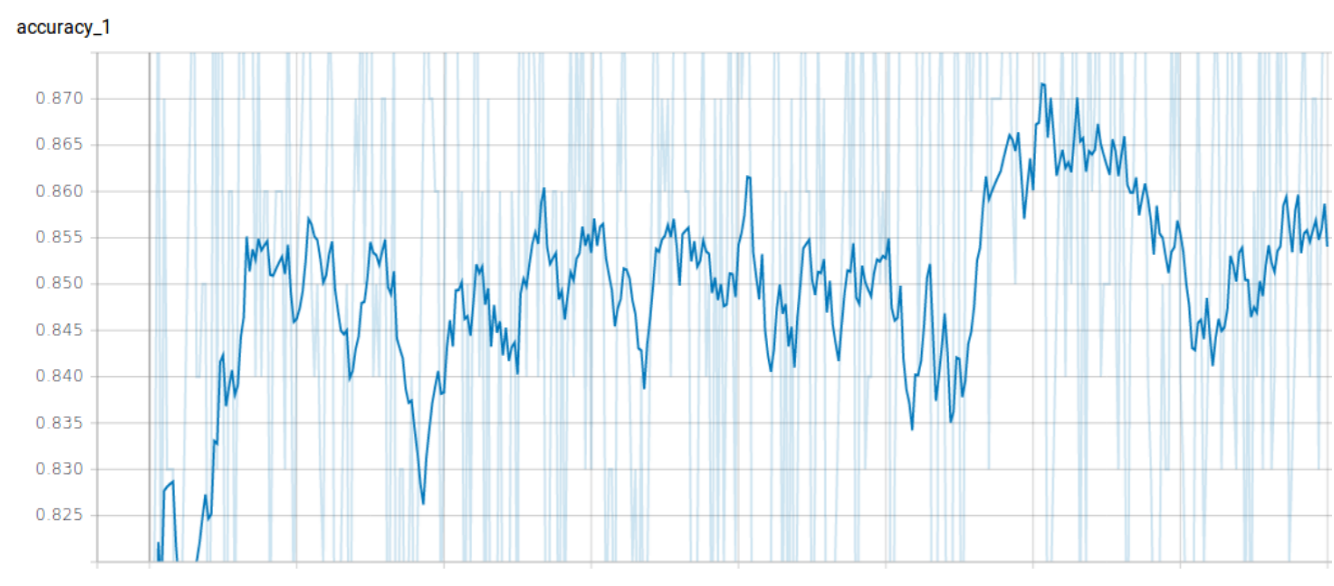
\includegraphics[scale=0.42]{transfer1.png}
    \caption{Résultats de la classification 31x31}
\end{figure}

\begin{figure}[H]
    \centering
    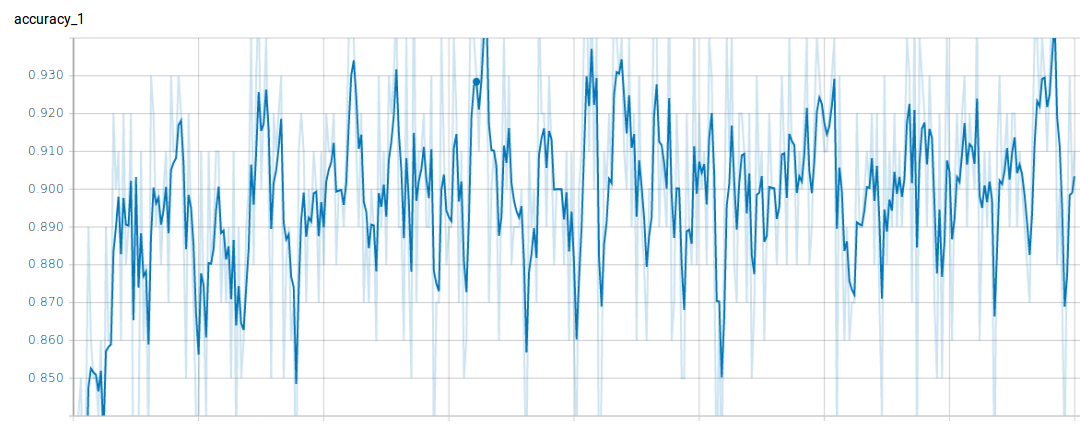
\includegraphics[scale=0.55]{transfer2.png}
    \caption{Résultats de la classification 99x99}
\end{figure}

Soit dans le premier cas, une accuracy finale de 0.855, contre 0.900 dans le second.

Nous n'avons pas obtenu de résultats de détection avec un réseau ré-entrainé.

\section{Utilisation d'un modèle plus complexe : Facenet}

Facenet est un outil de reconnaissance faciale, fondé sur un MTCNN (multi-task CNN) pré-entraîné pour la détection de visage. Nous avons utilisé une implémentation Tensorflow de l'article \href{https://arxiv.org/abs/1503.03832}{FaceNet: A Unified Embedding for Face Recognition and Clustering}

\subsection{Analyse qualitative des résultats}
\subsubsection{True positives}

Facenet a réussi à faire face à des situations compliquées, comme par exemple la détection de petits visages en arrière-plan ou de visages flous :

\begin{figure}[H]
    \centering
    \begin{minipage}[c]{0.45\linewidth}
        \begin{center}
            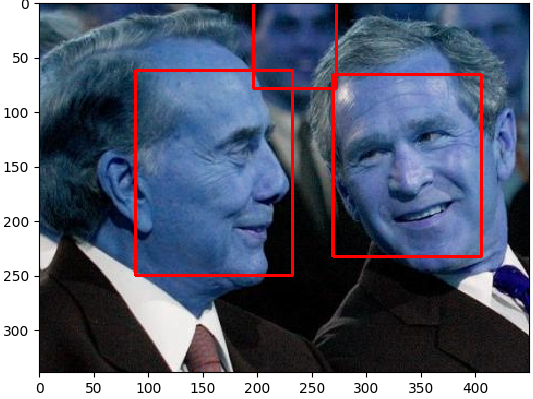
\includegraphics[scale=0.60]{facenetTP1.png}
            \caption{Détections de visages en arrière-plan}
        \end{center}
    \end{minipage} \hfill
    \begin{minipage}[c]{0.45\linewidth}
        \begin{center}
            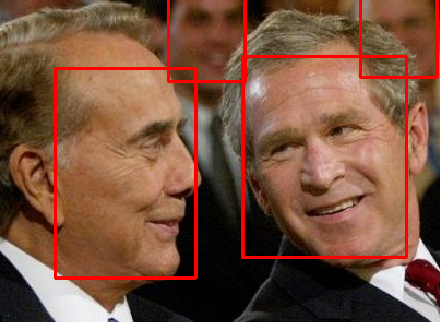
\includegraphics[scale=0.435]{facenetTP2.png}
            \caption{Détections de visages flous}
            \label{fig:proj_ecran}
        \end{center}
    \end{minipage}
\end{figure}

\subsubsection{False positives}

Par ailleurs, il y a des situations où la détection est erronée, mais pour lesquels on peut comprendre l'origine de l'erreur :\\

\begin{figure}[H]
    \centering
    \begin{minipage}[c]{0.45\linewidth}
        \begin{center}
            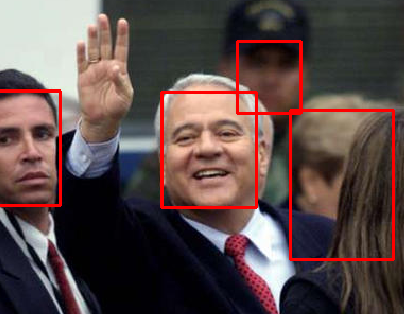
\includegraphics[scale=0.475]{facenetFP6.png}
            \caption{Faux positif lié à la présence d'un visage en tronqué (celui de droite)}
        \end{center}
    \end{minipage} \hfill
    \begin{minipage}[c]{0.45\linewidth}
        \begin{center}
            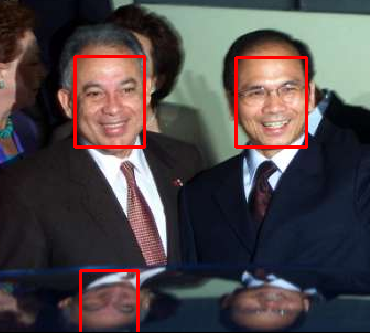
\includegraphics[scale=0.45]{facenetFP2.png}
            \caption{Faux positif lié au reflet du visage sur la table}
        \end{center}
    \end{minipage}
\end{figure}

\begin{figure}[H]
    \centering
    \begin{minipage}[c]{0.45\linewidth}
        \begin{center}
            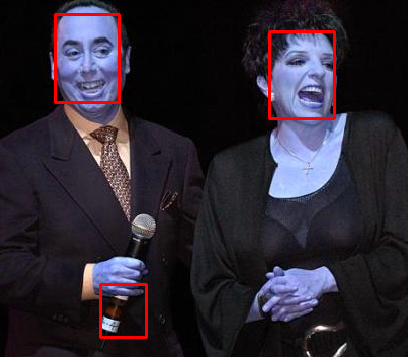
\includegraphics[scale=0.48]{facenetFP3.png}
            \caption{Faux positif lié à la détection de la statuette}
        \end{center}
    \end{minipage} \hfill
    \begin{minipage}[c]{0.45\linewidth}
        \begin{center}
            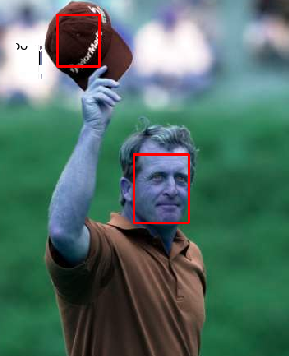
\includegraphics[scale=0.60]{facenetFP1.png}
            \caption{Faux positif lié à l'apprentissage de la corrélation visage-casquette}
            \label{fig:casquette}
        \end{center}
    \end{minipage}
\end{figure}

La figure \ref{fig:casquette} est en BGR, mais étant donné que le phénomène est intéressant et ne se produit pas en RGB nous avons gardé l'image.

Il y a également des faux positifs non explicables :\\

\begin{figure}[H]
    \centering
    \begin{minipage}[c]{0.50\linewidth}
        \begin{center}
            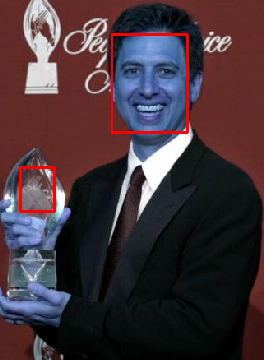
\includegraphics[scale=0.52]{facenetFP4.png}
            \caption{Faux positif inexplicable}
        \end{center}
    \end{minipage} \hfill
    \begin{minipage}[c]{0.45\linewidth}
        \begin{center}
            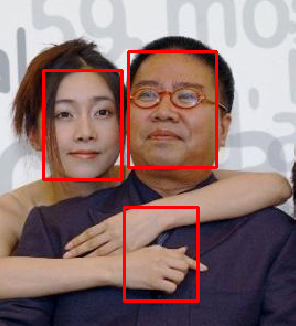
\includegraphics[scale=0.45]{facenetFP5.png}
            \caption{Faux positif inexplicable}
        \end{center}
    \end{minipage}
\end{figure}

\subsubsection{False negatives}

La très grande majorité des faux négatifs sont dus à des situations compliquées, comme des soucis de luminosité, des visages tronqués, ou des visages flous en arrière-plan.\\

\begin{figure}[H]
    \centering
    \begin{minipage}[c]{0.45\linewidth}
        \begin{center}
            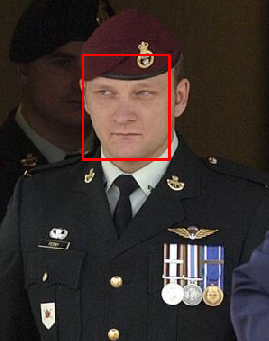
\includegraphics[scale=0.45]{facenetFN1.png}
            \caption{Faux négatif dû à la luminosité}
        \end{center}
    \end{minipage} \hfill
    \begin{minipage}[c]{0.45\linewidth}
        \begin{center}
            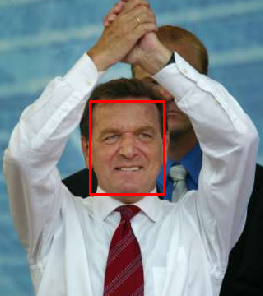
\includegraphics[scale=0.525]{facenetFN2.png}
            \caption{Faux négatif dû à un visage tronqué}
        \end{center}
    \end{minipage}
\end{figure}

\begin{figure}[H]
    \centering
    \begin{minipage}[c]{0.45\linewidth}
        \begin{center}
            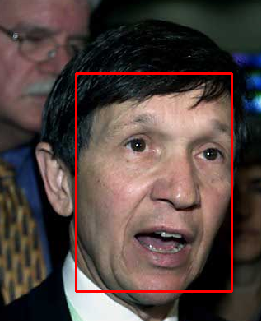
\includegraphics[scale=0.505]{facenetFN3.png}
            \caption{Faux négatifs dus aux deux visages tronqués}
        \end{center}
    \end{minipage} \hfill
    \begin{minipage}[c]{0.45\linewidth}
        \begin{center}
            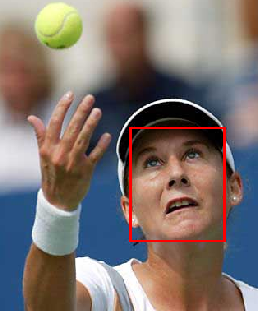
\includegraphics[scale=0.52]{facenetFN4.png}
            \caption{Faux négatifs dus au flou}
        \end{center}
    \end{minipage}
\end{figure}

\section{Complétion de la base de données d'entrée}
\label{sec:completion}
    
    \subsection{Nécessité de compléter la base de données}

	La nécessité d'augmenter la base de données provient du fait que la performance des
	algorithmes de deep learning est directement proportionnelle à la taille de la base de
	données (figure \ref{fig:data1}). Il est donc intéressant d'augmenter les données déjà présentes quand nous n'avons pas de donnée supplémentaire à utiliser.

	\begin{figure}[H]
	    \centering
	    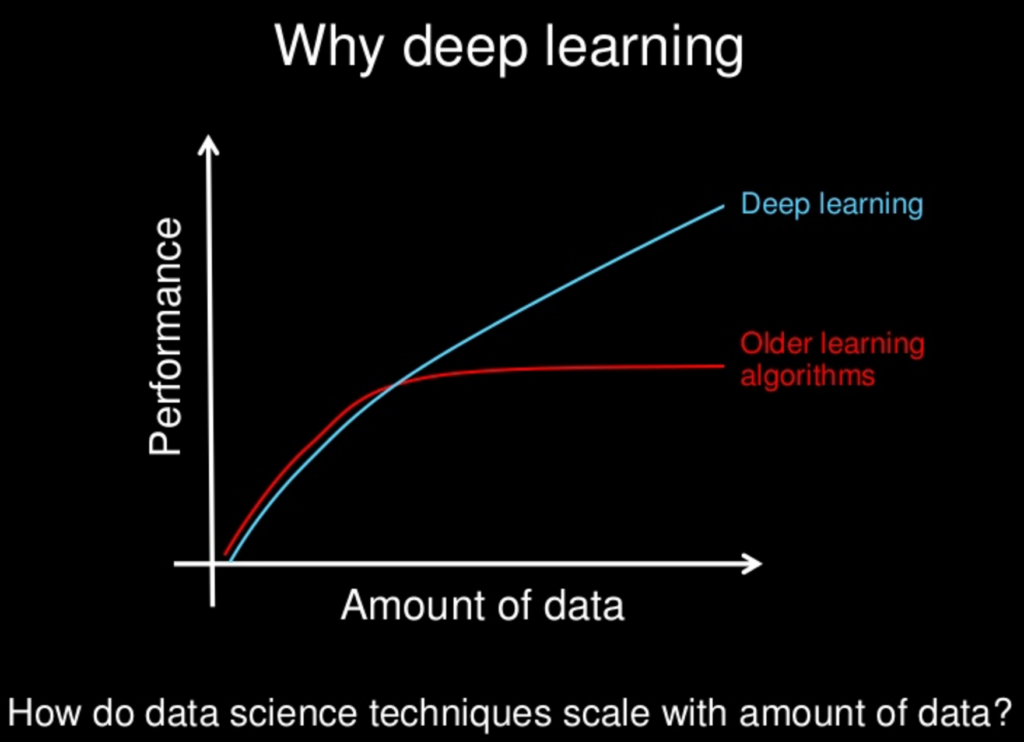
\includegraphics[scale=0.3]{deeplearning_data.png}
	    \caption{Graphe de performance en fonction du nombre de données}
	    \label{fig:data1}
	\end{figure}

    \subsection{Méthodes de complétion}

	Pour ce qui est des différentes méthodes d'augmentation, nous pouvons performer des
	transformations géométriques (translations, symétries, rotations) ou encore des
	déformations afin de reconnaître les photos prises avec des cameras "fisheyes".\\

	Il peut être intéressant d'altérer l'intensité de l'image de façon à reconnaître les images
	de test même si elles ont une amplitude d'intensité très variables. Nous pouvons par exemple
	citer la méthode de l'article AlexNet \cite{alexnet} qui prend l'intensité d'un pixel et lui
	rajoute un multiple des composantes principales de l'image (pour garder la valeur
	intrinsèque de l'image. Le multiple dépend des vecteurs propres de la matrice 3x3 de
	covariance du pixel et des valeurs propres de cette dernière multiplié par un coefficient
	de gaussienne de moyenne nulle et de variance $0.1$.\\

	Notre dernière idée consiste à appliquer un bruit blanc aux images afin de rendre
	l'algorithme moins sensible aux particularités d'une image mais plus au \textit{pattern}
	recherché.\\

	La représentation en RGB des images rajoute de la complexité (plus de dimensions) mais
	elle permet une meilleure performance du fait que la couleur humaine est particulière et se
	différencie grandement des couleurs d'arrière plan.

\newpage
\section{Annexes}
%http://ydwen.github.io/papers/WenECCV16.pdf
\bibliographystyle{unsrt}
\bibliography{sample}
%\flushleft [1] http://ydwen.github.io/papers/WenECCV16.pdf 
%[2] Zeiler, M. D., \& Fergus, R. (2014, September). Visualizing and understanding convolutional networks. In European conference on computer vision (pp. 818-833). Springer, Cham.

\end{document}
